\section{Theory}
In this section, the relevant theoretical background that is 
essential to the domain of Deep Reinforcement Learning will be introduced. 

\subsection{Reinforcement Learning}
RL is a method that is mostly used in dynamic game-like environments 
where an algorithm receives control of some actions and is required to learn a 
certain behavior \cite{RLBook}. Examples of this can be seen where agents apply RL algorithms to 
Atari games and achieve 
relatively high scores on a selection of them \cite{rlsolvingatari}. Being a type 
of machine learning, it employs a means to map situations to actions according to 
the maximization of a pre-determined numerical reward function \cite{RLBook}. The 
main process of learning is to adapt a decision maker, referred to as an agent, 
according to experiences. Here, an action is performed after which a reward is 
given in 
the form of a scalar value by the environment. 
All the externalities 
that determine what state the agent is in, is defined as the environment. This reward is 
then used as a cue  
to alter the mapping from states to actions accordingly. Using this process allows 
the agent to learn from experience on how to act in order to maximize its reward 
signal. The foundation of RL is based on the collaboration between the agent 
and the environment. For each time step, the agent 
finds itself in a certain state. During this state, the agent has a certain set 
of actions that it can choose from. For each of these actions, there 
is an effect on the environment. After performing a chosen action, the agent finds itself 
in a new state, repeating the process of action-selection. This loop is 
illustrated in Figure \ref{AgentEnv}. 

\begin{Figure}
    \centering
    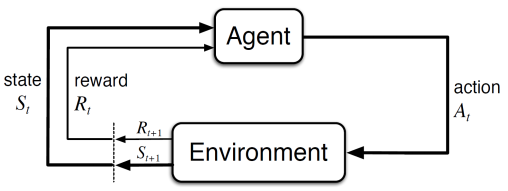
\includegraphics[width=0.8\linewidth]{literature/AgentEnv.png}
    \captionof{figure}[Agent-Environment interaction in RL]{Agent-Environment interaction in RL \cite{RLBook}}
    \label{AgentEnv}
\end{Figure}

The essence of this algorithm is based on the environment's response to each 
action from the agent. During training time, the environment gives 
the agent a reward, possibly in the form of a punishment. The function that 
determines this reward signal, is in turn what the agent will try to optimize and 
therefore, by definition, what the 
agent will try to learn \cite{RLBook}. 

To formalize this process, the agent takes a time-step $t$ which is defined to be a 
single sequence of 
state retrieval, action decision and new state retrieval. This is also written as 
$(S_t, A_t, R_{t+1}, S_{t+1})$.  In this sequence, the agent 
receives a state $S_t$ on which it decides on 
an action $a$ out of the possible available set of actions $A$ using a certain policy $\pi$.
Performing this action changes the environment and provides the agent with a 
new state: $S_{t+1}$. The environment also 
provides the agent with a reward $r_{t}$. By finding an optimal policy $a = \pi(s)$ 
that maximized this reward signal, the agent learns new behavior. An important aspect to consider 
for the agent, is the consideration 
of future rewards as well, which is 
recorded in the return $G_t$ of a certain action in a specific state. 
However, what actions will be chosen by the agent is dependent on the policy $\pi$
that the agent employs. The policy is defined as a probability distribution over
the possible actions for each state. Therefore, by defining an optimal policy 
that maximizes the return, the goal is achieved. 

A crucial concept in RL algorithms is the balance between exploration and exploitation \cite{RLBook}. 
When the policy is completely directed towards exploitation, the agent will 
not explore many of the other possible actions that can be taken that could 
potentially lead to higher returns. Instead, it simply tries to maximize its 
reward signal as much as possible from what it already knows about the world. However, 
there are potentially new states that the agent could explore that could yield 
higher returns. It would therefore be wise to explore the state-space some more. There is a 
strong interplay between exploration and exploitation during the training time of an 
agent that determines how much reward the agent will eventually be able to gather. 
The policies which perform the best are 
the ones that are able to balance both of these strategies in order to maximize 
the overall returns. 

\subsection{Q-Learning}
There are multiple ways in which to implement the learning algorithm in RL \cite{RLBook}. 
One of the more popular approaches, is the method of $Q$-learning. This 
method is characterized by keeping track of the value of performing each action during 
each state. Each action-state pair's value is defined to be the $Q$-value which 
is represented as the expected return for choosing an action $a$ in state $s$, 
expressed as $Q(s, a)=\mathbb{E}_{\pi}\left[R_{t} \mid s_{t}=s, a_{t}=a\right]$.
Intuitively, the expected return is the total sum of expected reward that will be 
collected by choosing this action and continuing from there onwards. This leads to 
the following simplified recursive equation:

\begin{equation}
    Q(s, a)=r+\gamma \max_{a^{\prime}} Q\left(s^{\prime}, a^{\prime}\right)
\end{equation}

The function of this equation in the context of $Q$-learning is, therefore, to update the 
$Q$-values throughout
the learning process where different action-state pairs are being explored. Since the agent, 
when just beginning, is unaware of what the values are for each action, it is imperative 
that it first probes the environment in order to explore the state-action space. The longer 
this process takes, the larger the size of explored state-action space is, and the more accurate 
the agent's predictions about the $Q$-values can be. 

Since $Q$-values represent the overall return of choosing
an action, this will create a mapping from each state to what the value is of each action in 
this state,
taking into account later state-action pairs. Having this information provides the algorithm 
with an overview of good and bad actions to take in each situation. By then employing a policy 
that 
chooses the action with the highest $Q$-value in each state, which is also called a greedy 
policy, 
the agent is able to maximize the reward signal.

\subsection{Deep Q-Learning}
In many RL applications, including the use of RL as a means to control a drone, there is the  
issue of how states and actions are represented. The implementation of Deep Q-Learning \cite{DQNDeepmind}
pose a solution to this problem, which will be discussed below.

In many domains where this algorithm 
is useful, the state or actions can be either continuous or discrete. In most discrete 
state-spaces, keeping a table of each $Q$-value for each state-action pair is a reasonable 
method to keep track of this information. However, in the case of 
a continuous space, keeping a tabular state-representation would vastly inflate the 
computational costs of 
storage, let alone searching time required to sift through this table. This means that 
there is a necessity 
to represent the action space, not categorically, but as a function. 

Additionally, in some applications, the state space is being represented as an image. Using 
images, which can take up a large range of values per pixel, can further complicate how the 
mapping of state to action values happens. However, more importantly, the location of 
the values become important. Image processing requires the processing of the interrelated 
connections between pixels in its 2-dimensional spaces. These problems necessitate 
different requirements to the function approximation tasks compared to a simple one-dimensional 
state input. \newline

\noindent
\textbf{Convolutions and Neural Networks} \newline 
Neural networks have previously been used in order to perform function 
approximations, especially in the context of RL \cite{rlsolvingatari}. Neural networks 
are a biologically inspired network of digital neurons that make predictions and 
adapt accordingly when presented with a ground truth \cite{neuralnets}. The building 
blocks, the neurons 
themselves, have weighted connections to other neurons. These connections 
are the weighted sums of their inputs and a bias term. During initialization of such 
a network, all of these values, also called parameters, are random. The training process 
is defined by the 
modification of these weights and bias terms in order to fit to the data that it is 
being fed. This process happens by the network producing an output prediction, which 
is then checked according to a ground truth. Using the difference between this ground truth and 
the prediction, a cost value is produced and thereby, a cost function. 
An algorithm is then used that calculates the gradient of the parameters that will minimize 
this cost function, which is also referred to as backpropagation. During a training cycle, 
a batch of data is fed forward through a network 
and a gradient towards better weights and biases is calculated and applied. Iterating 
this process, modifies the network to adapt to the data. More importantly, this 
also provides the network with the ability to generalize to new, yet unfamiliar 
data points. There is a strong trade-off regarding the degree to which  a neural 
network has been fitted to training data. The more the network adapts, the better it 
fits the data and can generalize. Nevertheless, it is possible to overdo this, causing 
the network to fit to the data too much, losing its generalization abilities. This 
phenomenon is called overfitting.  

Using neural networks has been an extremely useful tool in many 
domains \cite{riseofneuralnets, NeuralNetworkApplications}. One such domain is 
computer vision, which deals with different vision tasks such as 
visual recognition, image classification, object localization, and object detection 
\cite{CNNapplications2}. Some of these tasks have seen drastic improvements with the 
introduction of a specific type of neural network called a Convolutional Neural 
Network (CNN) \cite{CNNapplications, CNNintroduction, firstcnn}. CNNs rely on the 
principle of convolutions as an operation on the input. This convolution employs a filter 
(also referred to as a kernel) which is a matrix that is applied to the input pixels as a 
sliding window. Performing this operation on the input, creates a new image which 
extracts specific features, dependent on the filter being applied. In the case of 
a CNN, the goal is to learn relevant filters to be applied on the input, in order 
to make correct predictions. The final layers of a CNN mostly consist of fully 
connected layers, which are identical to the normal neural network architecture as 
described earlier. CNN architectures output a probability distribution 
over all the available classes, where the highest probability class is chosen 
as a prediction. 

The application of neural networks as function approximators in RL has been 
a popular choice \cite{rlanoverview}, but especially so in the case of 
$Q$-learning. The determination process of the state-action pairs and their 
corresponding $Q$-values can be performed using the CNN. 
Instead of a class distribution, the CNN now outputs predictions about 
the $Q$-values of each available action, forming this value approximation method.
By employing a certain policy using these values, different behaviors can now 
be either found or performed.   \newline


\noindent
\textbf{Deep Q-Network} \newline
The combination of using both a CNN (or any other type of neural network as a function 
approximator), as a $Q$-learning algorithm is called Deep Q-Learning. An agent 
employing this is called a Deep Q-Network (DQN) \cite{DQNDeepmind} and
works similar to a normal $Q$-learning algorithm. The agent gathers 
experiences in a certain environment, and stores these experiences in a 
replay buffer. During training time, it samples a batch from this 
replay buffer and performs the feed forward through the CNN. Using the  
outputs from the network to compare against what was actually 
observed during the batch of experiences. With this difference, a gradient 
can be calculated which can be backpropagated through the network to become more 
accurate in its $Q$-value predictions. Iterating this process eventually ensures 
that the agent converges at either a local or global minimum. 
Using samples of experiences as training data is done for a more stable training process 
because a possible danger of using only the latest acquired experiences is that the agent 
will forget learned behavior from older experiences degrading its performance.  Furthermore,
changes in parameters also mean changes in behavior, which leads to new experiences 
and consequently, a bias in the data. The fact that the training batches will always 
contain a proportion of considerably older experiences, assures that the agent will always 
be updated with those experiences as well, enabling overall more stable a training 
process.

Once a DQN has been trained, policy selection is straight-forward because a 
greedy policy can be applied to maximize the current knowledge about the reward 
space. However, during training time, to be able to tweak the 
exploration-exploitation process, an $\epsilon$-greedy policy can be applied. 
This policy selects the actions 
with the highest $Q$-value, expect for an $\epsilon$ proportion of times, 
where a random action is chosen. Maintaining an amount of randomness during 
action selection during training time, ensures that at least some degree 
of exploration will be present. Once the training process has been finished, 
this $\epsilon$ can be reduced to naught, prioritizing exploitation. 
